\chapter{Metodologia}

Metodologias específicas colaboram para estabelecer diretrizes e boas práticas na condução do trabalho, conferindo padronização, noções de pesquisa científica, dentre outras contribuições \cite{Wohlin:2000}.

A metodologia pode ser entendida como um conjunto de etapas a serem realizadas na condução do processo investigativo em um determinado contexto. É a metodologia que define os passos que serão seguidos para realização das pesquisas, escolha do tema, planejamento da investigação, desenvolvimento, coleta e análise dos dados, análise dos resultados e conclusões a respeito das lições aprendidas\cite{Moresi:2003}.

Pesquisar significa identificar uma dúvida que necessite ser esclarecida, construir e executar o processo que apresenta a solução desta, quando não há teorias que a expliquem ou quando as teorias que existem não estão aptas para fazê-lo \cite{Koche:1997}. A seguirão apresentadas as formas de se classificar uma pesquisa.

\section{Classificação da pesquisa}

\begin{itemize}
	\item Do ponto de vista da natureza da pesquisa, esta pode ser:
		\begin{itemize}
			\item \textbf{Pesquisa Básica:} Possui o objetivo de gerar novos conhecimentos para a ciência. Neste tipo de pesquisa não é obrigatório que o conhecimento gere um uso prático \cite{Silva:Tafner:2007}.
			\item \textbf{Pesquisa Aplicada:} Visa gerar uma maior compreensão para assuntos práticos dirigidos à solução de problemas específicos \cite{Silva:Tafner:2007}.
		\end{itemize}

	\item Do ponto de vista da forma de abordagem do problema,tem-se:
		\begin{itemize}
			\item \textbf{Pesquisa Quantitativa:} O estudo quantitativo considera que tudo pode ser quantificável, ou seja, que os números podem ser classificados, gerando informações ao analisá-los, através da análise estatística \cite{Travassos:2002}.
			\item \textbf{Pesquisa Qualitativa:} O estudo qualitativo está relacionado à pesquisa sobre os objetos, quando os resultados são apresentados em termos naturais, usando conjuntos nebulosos, porcentagens de satisfação, dentre outras formas de classificar algo subjetivo \cite{Travassos:2002}.
		\end{itemize}

	\item Do ponto de vista de seus objetivos, tem-se:
		\begin{itemize}
			\item \textbf{Pesquisa Exploratória:} Esta pesquisa tem como objetivo proporcionar maior familiaridade com o problema, possibilitando o aprimoramento de ideias ou a descoberta de intuições \cite{Gil:2010}.
			\item \textbf{Pesquisa Descritiva:} Seu principal objetivo é a descrição das características de determinada população ou fenômeno ou, então, o estabelecimento de relações entre variáveis \cite{Gil:2010}.
			\item \textbf{Pesquisa Explicativa:} Tem como preocupação central identificar os fatores que determinam ou que contribuem para a ocorrência dos fenômenos. Esse é o tipo de pesquisa que mais aprofunda o conhecimento da realidade, porque explica a razão, o porquê das coisas \cite{Gil:2010}.
		\end{itemize}

	\item Do ponto de vista dos procedimentos técnicos, pode ser:
		\begin{itemize}
			\item \textbf{Pesquisa Bibliográfica:} Visa encontrar as fontes primárias e secundárias e os materiais científicos e tecnológicos necessários para a realização do trabalho científico ou técnico-científico. Muitos estudos fazem uso do levantamento bibliográfico ou são desenvolvidas exclusivamente por fontes bibliográficas. Sua principal vantagem é possibilitar ao investigador a cobertura de uma gama de acontecimentos muito ampla \cite{Silva:Tafner:2007}.

			\item \textbf{Pesquisa Documental:} Assemelha-se à pesquisa bibliográfica. Porém, esta é realizada a partir de materiais que não receberam tratamento analítico. Por exemplo, reportagens de jornal, cartas, contratos, diários, filmes, fotografias e gravações. A pesquisa documental pode ser realizada ainda através de documentos de segunda mão, que de alguma forma já foram analisados. Por exemplo, relatórios de empresas e tabelas estatísticas \cite{Gil:2010}.

			\item \textbf{Levantamento:} É uma investigação realizada em retrospecto, que em seguida, mediante análise quantitativa, chega as conclusões correspondentes aos dados coletados. O levantamento feito com informações de todos os integrantes do universo da pesquisa origina um censo. \cite{Mafra:Travassos:2006}.
			
			\item \textbf{Estudo de Caso:} São estudos conduzidos com o propósito de se investigar uma entidade ou um fenômeno dentro de um espaço de tempo específico. Estes são usados principalmente para a monitoração de atributos presentes em projetos, atividades ou atribuições. Durante a sua condução, dados são coletados e analisados estatisticamente de forma a permitir a avaliação de um determinado atributo ou do relacionamento entre diferentes atributos. \cite{Mafra:Travassos:2006}
			
			\item \textbf{Pesquisa-Ação:} É realizada em conjunto com uma ação ou com a resolução de um problema coletivo, visando definir o campo de investigação, as expectativas dos interessados e o tipo de auxílio que estes poderão exercer ao longo do processo de pesquisa. Esta pesquisa implica no contato direto com o campo de estudo, envolvendo o reconhecimento visual do local, consulta a documentos diversos e a discussão com os envolvidos na pesquisa. A abordagem dos problemas dos grupos investigados na pesquisa-ação é mais qualitativa do que quantitativa \cite{Silva:Tafner:2007}.
			
			\item \textbf{Pesquisa Participante:} A intenção é obter um maior conhecimento sobre o grupo. O grupo investigado tem ciência da finalidade, dos objetivos da pesquisa e da identidade do pesquisador. A pesquisa participante permite a observação das ações no próprio momento em que ocorrem \cite{Silva:Tafner:2007}.
			
			\item \textbf{Pesquisa Experimental:} É conduzida quando deseja-se obter um maior controle da situação, ao se manipular as variáveis envolvidas no estudo de forma direta, sistemática e precisa. A pesquisa experimental necessita de previsão de relações entre as variáveis a serem estudadas, como também o seu controle. O objetivo é manipular uma ou mais variáveis e controlar todas as outras variáveis em um valor fixo. O efeito da manipulação das variáveis é então medido e, baseado nessa medição, análises estatísticas são conduzidas. A condução de experimentos reais é rara em Engenharia de Software, devido à dificuldade de se alocar os participantes do estudo a diferentes tratamentos de forma aleatória. Nessas situações, tais estudos denominam-se quasi-experimentos \cite{Mafra:Travassos:2006}.
			
			\item \textbf{Pesquisa Ex-Post-Facto:} Realizada quando o experimento se dá depois dos fatos. Neste caso, o pesquisador não tem controle sobre as variáveis. Esta pesquisa difere da pesquisa experimental pelo fato de o fenômeno ocorrer naturalmente sem que o pesquisador tenha controle sobre ele, ou seja, o pesquisador passa a ser um mero observador do acontecimento \cite{Silva:Tafner:2007}.
		\end{itemize}

\end{itemize}

\section{Planejamento da Metodologia Aplicada}

Este trabalho possui metodologias específicas para a realização do levantamento bibliográfico e do desenvolvimento das aplicações propostas.

A seguir serão apresentadas as duas metodologias e como estas serão aplicadas ao logo deste trabalho.

\subsection{Metodologia de Pesquisa}

Analisando-se o tema proposto para este trabalho pode-se ver que a pesquisa caracteriza uma pesquisa aplicada, pois, todo levantamento bibliográfico visa a geração de compreensões a cerca dos temas e estes conhecimentos adquiridos deverão ser aplicados no desenvolvimento. A abordagem é tanto quantitativa quanto qualitativa.

Com relação aos objetivos da pesquisa, considera-se que é uma pesquisa exploratória, devido à necessidade encontrada em entender mais adequadamente o problema apresentado e se obter um melhor entendimento de todos os temas relacionados ao que se propõe.

Por fim, no contexto dos procedimentos técnicos, será aplicada a pesquisa bibliográfica visando o levantamento de uma ampla gama de fontes para se alcançar o conhecimento necessário para a realização do trabalho. Além da pesquisa exploratória, tem-se também a aplicação da pesquisa-ação.

\subsection{Metodologia de Desenvolvimento}

A metodologia de desenvolvimento seguirá algumas práticas ágeis já consolidadas. Basicamente, pretende-se utilizar as práticas ágeis propostas na metodologia \textit{Scrum}\footnote{\url{http://www.desenvolvimentoagil.com.br/scrum/}}, com o uso de estórias de usuário, reuniões diárias, \textit{sprints} de quinze dias, \textit{backlog do produto} e \textit{backlog de sprint}. Serão aplicadas também algumas práticas do \textit{XP}\footnote{\url{http://www.desenvolvimentoagil.com.br/xp/}}, como o uso de integração contínua, pareamento e \textit{planning poker} para estimativa de pontos das estórias.

\subsection{Fluxo De Trabalho}

A Figura \ref{processo tcc} apresenta o fluxo de trabalho que orientará a condução desse trabalho.

\newpage

\begin{figure}
	\centering
	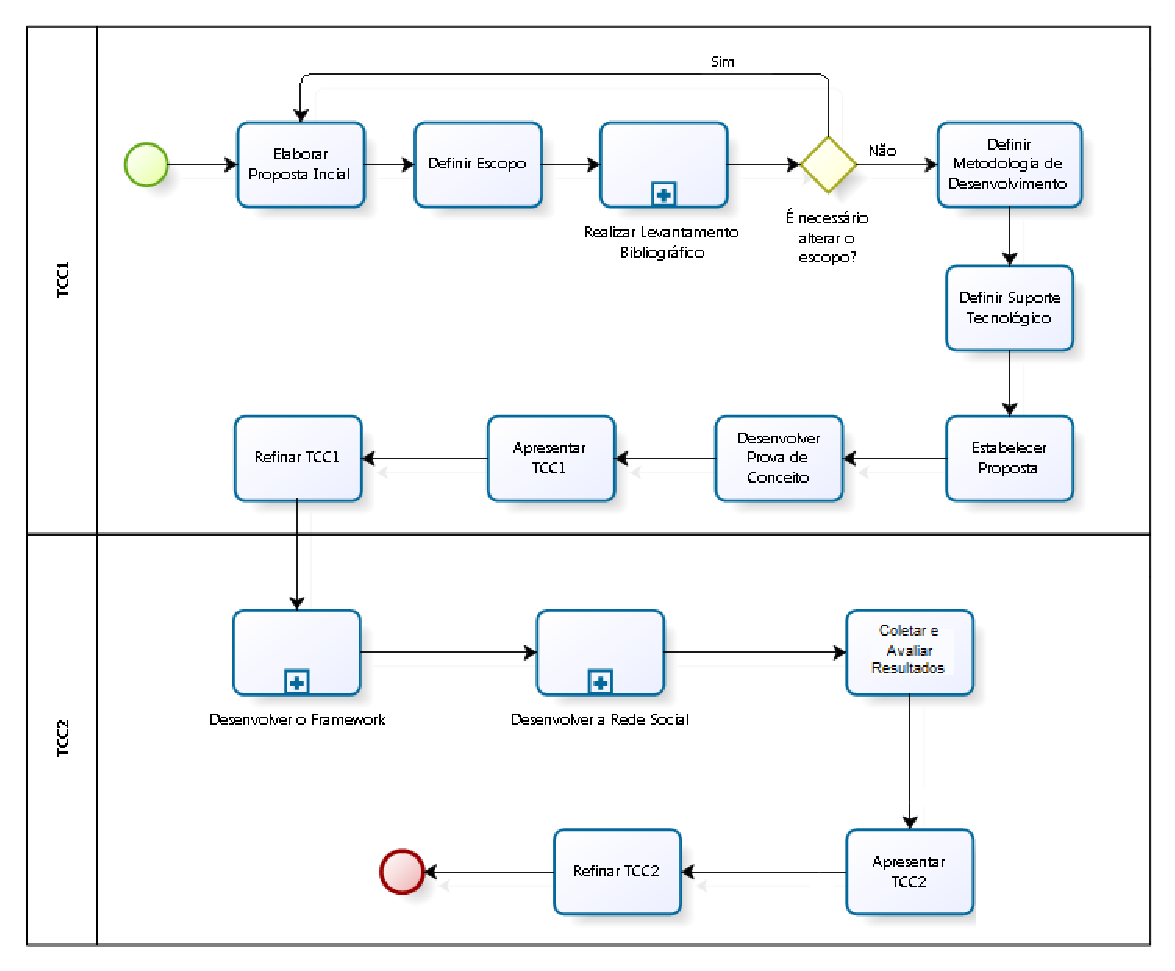
\includegraphics[scale=0.8]{figuras/capitulo4/processo_tcc.eps}
	\caption{Fluxo de trabalho}
	\label{processo tcc}
\end{figure}

O fluxo apresentado mostra a distribuição das principais atividades que ou já foram realizadas (caso sejam do escopo do TCC1), ou serão realizadas (em se tratando de atividades no escopo do TCC2). Primeiramente, a ideia inicial para o projeto é definida bem como trabalhada, obtendo como resultado a proposta (em seu esboço preliminar). A partir dessa proposta, o escopo inicial é definido, conferindo base para a realização do levantamento bibliográfico. Ao final, caso haja necessidade, volta-se o fluxo ao início, visando um melhor refinamento do que já foi realizado.

A partir da proposta inicial, são definidos a metodologia de desenvolvimento, o suporte tecnológico e uma proposta mais concreta, a qual será de fato desenvolvida ao longo do TCC. Para comprovar a viabilidade da proposta, uma prova de conceito deve ser elaborada.

Por fim, o trabalho deve ser apresentado e refinado de acordo com as observações da banca examinadora.

A segunda parte do fluxo apresenta as atividades relacionadas ao desenvolvimento do framework e da rede social que usará este framework, comprovando assim a sua instanciação e aplicabilidade. Na última etapa os, resultados obtidos são coletados e o trabalho final é apresentado e refinado.

\subsection{Cronograma}

A seguir são apresentados os cronogramas preliminares referentes às atividades que serão realizadas durante todo este trabalho. Estes cronogramas estão dividos entre as atividades das etapas um (que abrangem o período entre agosto de 2015 e janeiro de 2016) e dois (que abrangem o período entre março e junho de 2016).

\begin{table}[h]
\centering
\caption{Cronograma do TCC1}
\label{cronograma tcc1}
\begin{adjustbox}{width=\textwidth}
\begin{tabular}{|l|c|c|c|c|c|c|}
\hline
                                      			& \multicolumn{1}{l|}{\textbf{Agosto}} & \multicolumn{1}{l|}{\textbf{Setembro}} & \multicolumn{1}{l|}{\textbf{Outubro}} & \multicolumn{1}{l|}{\textbf{Novembro}} & \multicolumn{1}{l|}{\textbf{Dezembro}} \\ \hline
\textbf{Elaborar Proposta Inicial}              & X                           		   &                               			&                              			&                               		 &                               		  \\ \hline
\textbf{Definir Escopo}                         & X                           		   &                               			&                              			&                               		 &                               		  \\ \hline
\textbf{Realizar Levantamento Bibliográfico}    & X                           		   & X                             			&                              			&                               		 &                               		  \\ \hline
\textbf{Definir Metodologia} 					&                             		   & X                             			& X                            			&                               		 &                               		  \\ \hline
\textbf{Definir Suporte Tecnológico}            &                             		   &                               			& X                            			&                               		 &                               		  \\ \hline
\textbf{Estabelecer Proposta}                   &                             		   &                               			& X                            			& X                             		 &                               		  \\ \hline
\textbf{Desenvolver Prova de Conceito}          &                             		   &                               			&                              			& X                             		 &                               		  \\ \hline
\textbf{Apresentar TCC1}                        &                             		   &                               			&                              			& X                              		 &                              		  \\ \hline
\textbf{Refinar TCC1}                           &                             		   &                               			&                              			&                               		 & X                              		  \\ \hline
\end{tabular}
\end{adjustbox}
\end{table}

\begin{table}[h]
\centering
\caption{Cronograma do TCC2}
\label{cronograma tcc2}
\begin{tabular}{|l|c|c|c|c|c|c|}
\hline
                                      			& \multicolumn{1}{l|}{\textbf{Março}} & \multicolumn{1}{l|}{\textbf{Abril}} & \multicolumn{1}{l|}{\textbf{Maio}} & \multicolumn{1}{l|}{\textbf{Junho}} & \multicolumn{1}{l|}{\textbf{Julho}} \\ \hline
\textbf{Desenvolver o Framework}                & X                           		  & X                              		& X                            		 &                               	   &                               		 \\ \hline
\textbf{Desenvolver a Rede Social}              &                            		  &                               		& X                            		 & X                              	   &                               		 \\ \hline
\textbf{Elaborar Resultados}				    &                            		  &                              		&                             		 & X                             	   &                               		 \\ \hline
\textbf{Apresentar TCC2}						&                             		  &                              		&                             		 & X                              	   &                               		 \\ \hline
\textbf{Refinar TCC2}				            &                             		  &                               		&                             		 &                               	   & X                             		 \\ \hline
\end{tabular}
\end{table}

\section{Resumo do Capítulo}

Este capítulo apresentou as metodologias que serão utilizadas durante a realização das pesquisas e do desenvolvimento do projeto proposto.

Inicialmente, foram apresentadas diversas metodologias já conhecidas e que são usadas para diferentes trabalhos. Essas metodologias estão divididas de acordo com o ponto de vista da natureza da pesquisa, da forma de abordagem, dos objetivos e dos procedimentos técnicos. Com a apresentação de todas as metodologias, foram selecionadas as que melhor se adequam a este trabalho. A metodologia de desenvolvimento segue práticas ágeis e está baseada no Scrum.

Foi apresentado também o fluxo de trabalho com as atividads definidas para as duas etapas de desenvolvimento deste trabalho e bem como o cronograma proposto inicialmente para cumprimento destas atividades.

O próximo capítulo apresentará a proposta consolidada, que irá mostrar de fato qual o propósito e o que será desenvolvido e entregue ao final.
